\chapter{Introduction}
\section{Background}
We have to say that law plays a very important role in our humans' lives, Law is a system of rules that are created and enforced through social or governmental institutions to regulate behavior.
Law as a system helps regulate and ensure that a community show respect, and equality among themselves. It is a huge system which holds different kinds of aspects such as maintaining equality, punishing the sinner, Coordination of disputes, etc. It is the rule of human society.
\begin{figure}[!h]
\centering
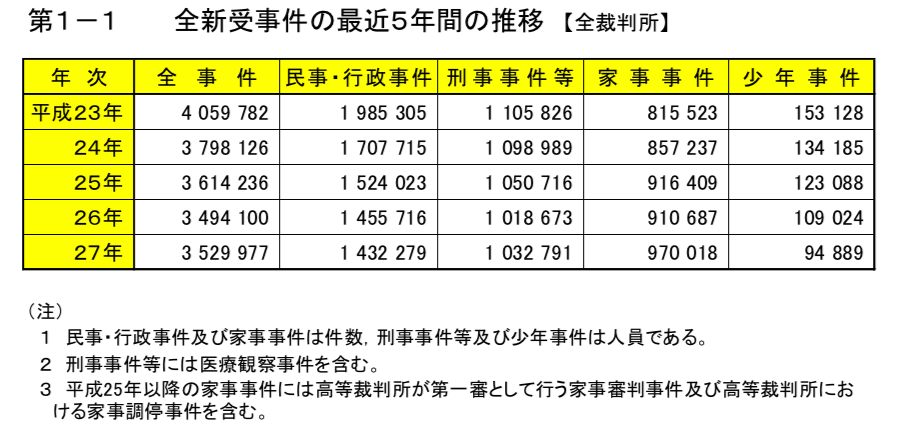
\includegraphics[width=350pt]{./pictures/0101.png}
\caption{information of cases accepted by all courts in Japan}
\end{figure}
\\At the present time, People always would like to use the law to protect their rights, besides civil cases, commercial cases, or even criminal cases. More and more people are dealing with family disputes through legal means. According to the newest data of Court of Japan(Http://www.courts.go.jp)[2], 3529977 new cases have been accepted by different courts, besides local courts, and the supreme court in H.27. The number of family cases accepted is increased by 18.9\% from 815523 cases to 970018 cases during the past five years (data of H.23 to H.27).
\\
Although we know old precedents is very helpful for new cases, there is also a fact that precedents are very long and very difficult to understand for our laymen. It is also not an easy work for specialists to find similar points among numbers of old precedents in a short time.
\\
Hard back to our subject, we want to propose a workable method, which should be easily accessed, highly efficient, to find descriptive similarity points among numbers of precedents.
\begin{figure}[!h]
\centering
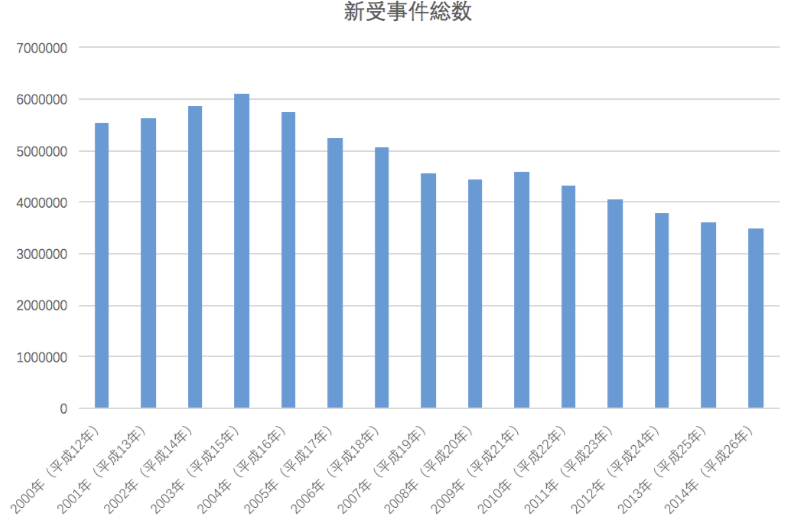
\includegraphics[width=400pt]{./pictures/0101-1.png}
\caption{the number of new litigations in recent years}
\end{figure}